%% ============================================================================
%%
%%  Speciale / Master's thesis
%%
%%  Author: FORNAVN EFTERNAVN
%%
%%  IMPORTANT: Compile with pdfLaTeX+biber !
%%
%%  Remarks:
%%  - Needs to be executed with '--shell-escape' if the minted-package is used!
%%
%%  Original template/preamble: Jakob Lysgaard Rørsted (Mosumgaard)
%% ============================================================================

% ~~~~~~~~~~~~~~~~~~~~~~~~~~~~~~~~~~~~~~~~~~~~~~~~~~~~~~~~~~~~~~~~~~~~~~~~~~~~~
% Preamble and input control
% ~~~~~~~~~~~~~~~~~~~~~~~~~~~~~~~~~~~~~~~~~~~~~~~~~~~~~~~~~~~~~~~~~~~~~~~~~~~~~

% Use memoir!!!
\documentclass[%
% final,           % Un-comment when finished (to e.g. remove watermark)
11pt,
openright,
twoside,
% danish,
british,
a4paper
]{memoir}

% Global definition: Name of the project (e.g. for the headers)
% NOTE: The text of the front page is defined manually!
\newcommand{\projecttitle}{Big Bang Nucleosynthesis}
\newcommand{\projecttitledanish}{Big Bang Kernesyntese}

% Read the actual preamble
%% ============================================================================
%%
%%  Master's thesis
%%
%%  Author: FORNAVN EFTERNAVN
%%
%%  Preamble
%%
%%  Original preamble: Jakob Lysgaard Rørsted (Mosumgaard)
%% ============================================================================

% ~~~~~~~~~~~~~~~~~~~~~~~~~~~~~~~~~~~~~~~~~~~~~~~~~~~~~~~~~~~~~~~~~~~~~~~~~~~~~
% Core
% ~~~~~~~~~~~~~~~~~~~~~~~~~~~~~~~~~~~~~~~~~~~~~~~~~~~~~~~~~~~~~~~~~~~~~~~~~~~~~
% Essentials
\usepackage[utf8]{inputenc}
\usepackage[T1]{fontenc}

% Microtype -- Subliminal refinements towards typographical perfection
\usepackage{microtype}
\microtypesetup{final}
% \microtypesetup{tracking = true}

% Various tools needed in the preamble and by some packages
\usepackage{etoolbox}

% Inclusion of code
% --> Needs to be loaded this early to avoid problems with some font packages
% NOTE: This packages requires the Python-module 'Pygments' to be installed
% NOTE: Fails unless this file is compiled with '--shell-escape' !
% \usepackage{minted}
% \usemintedstyle{friendly}

% Language (has to be loaded before the fonts..?)
% Load both languages to make two different abstracts
\usepackage[danish,english]{babel}
%\usepackage[danish,british]{babel}
\renewcommand\danishhyphenmins{22}
\selectlanguage{english}

% Fonts: Linux Libertine (http://www.tug.dk/FontCatalogue/linuxlibertine/)
\usepackage{libertine}            % Linux Libertine as text font
\usepackage{libertinust1math}     % Math support for Linux Libertine
\usepackage[scaled=.95]{newtxtt}  % Pretty teletype in correct size


% ~~~~~~~~~~~~~~~~~~~~~~~~~~~~~~~~~~~~~~~~~~~~~~~~~~~~~~~~~~~~~~~~~~~~~~~~~~~~~
% Page 'n' stuff
% ~~~~~~~~~~~~~~~~~~~~~~~~~~~~~~~~~~~~~~~~~~~~~~~~~~~~~~~~~~~~~~~~~~~~~~~~~~~~~
% Page set-up
\setlrmarginsandblock{3.2cm}{*}{1.5}
\setulmarginsandblock{*}{3.7cm}{1}

% Some memoir tricks
\setlength{\topskip}{1.6\topskip}
\checkandfixthelayout
\sloppybottom
\strictpagechecktrue

% To remove the blank page after the titlepage to save space
% --> Only for this progress report! Normally the blank page should be there!!
\usepackage{atbegshi}


% ~~~~~~~~~~~~~~~~~~~~~~~~~~~~~~~~~~~~~~~~~~~~~~~~~~~~~~~~~~~~~~~~~~~~~~~~~~~~~
% Page and chapter styles
% ~~~~~~~~~~~~~~~~~~~~~~~~~~~~~~~~~~~~~~~~~~~~~~~~~~~~~~~~~~~~~~~~~~~~~~~~~~~~~

% NOTE: Colors added everywhere, to make them easy to change!
\usepackage{xcolor}

% Fonts
\newcommand{\foliofont}{\color{black}\sffamily}
\newcommand{\headerfont}{\color{black}\sffamily}

% Make new pagestyle
\makepagestyle{jrmbsc}
\makeevenhead{jrmbsc}{\foliofont\thepage}    {} {\headerfont\leftmark}
\makeoddhead {jrmbsc}{\headerfont\projecttitle} {} {\foliofont\thepage}
\makeevenfoot{jrmbsc}{}{}{}
\makeoddfoot {jrmbsc}{}{}{}

% Black magic happens below! (define pagestyle)
\makeatletter
\makepsmarks {jrmbsc}{
  % Syntax: \createmark{<division type}{left|right|both marks}{shownumber|nonumber}{prefix}{postfix}
  \createmark{chapter}    {both}  {shownumber} {\@chapapp\ } {\ $\cdot$\ }
  \createmark{section}    {right} {shownumber} {}            { \ }
%  \createmark{subsection} {right} {nonumber}   {}            {}
  \createplainmark{toc}   {both}  {\contentsname}
  \createplainmark{lof}   {both}  {\listfigurename}
  \createplainmark{lot}   {both}  {\listtablename}
  \createplainmark{bib}   {both}  {\bibname}
  \createplainmark{index} {both}  {\indexname}
}
\makeatother
\nouppercaseheads

% Sections with sans-serif
\setsecheadstyle{\Large\bfseries\sffamily\raggedright}
\setsubsecheadstyle{\large\bfseries\sffamily\raggedright}

% Fix of the pagestyle of the chapter-pages
\copypagestyle{chapter}{empty}
\makeoddfoot{chapter}{}{\foliofont\thepage}{}
\makeevenfoot{chapter}{}{\foliofont\thepage}{}

% Chapterstyle (modified from Rasmus Villemoes thesis)
\usepackage{graphicx}
\makechapterstyle{jrmbsc}{% requires graphicx package
  \chapterstyle{default}
  \renewcommand*{\chapnamefont}{%
    \normalfont\LARGE\color{black}\scshape\raggedleft}
  \renewcommand*{\chaptitlefont}{%
    \normalfont\Huge\color{black}\sffamily\raggedleft}
  \renewcommand*{\chapternamenum}{}
  \renewcommand*{\printchapternum}{%
    \makebox[0pt][l]{\hspace{0.4em}
      \resizebox{!}{5ex}{%
        \normalfont\Large\color{black}\thechapter}
    }%
  }%
  \renewcommand*{\afterchapternum}{%
    \par\hspace{1.5cm}\color{black}\hrule\vskip\midchapskip}}

% Use the new pagestyle and chapterstyle
\pagestyle{jrmbsc}
\chapterstyle{jrmbsc}

% Turn on numbering of subsections
\setsecnumdepth{subsection}


% ~~~~~~~~~~~~~~~~~~~~~~~~~~~~~~~~~~~~~~~~~~~~~~~~~~~~~~~~~~~~~~~~~~~~~~~~~~~~~
% Floats, captions and footnotes
% ~~~~~~~~~~~~~~~~~~~~~~~~~~~~~~~~~~~~~~~~~~~~~~~~~~~~~~~~~~~~~~~~~~~~~~~~~~~~~
% Include graphics
% \usepackage{graphicx}  % ALREADY IMPORTED

% Subfloats
\newsubfloat{figure}
\subcaptionstyle{\raggedright}

% Use sans-serif for captions (alternative layout: Change width (see below))
\captionnamefont{\sffamily\scshape}
\captiontitlefont{\sffamily\small}

% Width of caption --> Use sf-font instead
% \captionwidth{.8\linewidth}
% \changecaptionwidth

% Trick to automatically end captions with a period
\captiontitlefinal{.}

% Styling of the footnotes (memoir tricks)
\setlength{\footmarkwidth}{-1sp}
\setlength{\footmarksep}{0em}
\footmarkstyle{#1: }

% Cool tables with footnotes (using the same style as define just above)
\usepackage[online]{threeparttable}
\appto\TPTnoteSettings{\footnotesize}


% ~~~~~~~~~~~~~~~~~~~~~~~~~~~~~~~~~~~~~~~~~~~~~~~~~~~~~~~~~~~~~~~~~~~~~~~~~~~~~
% Science
% ~~~~~~~~~~~~~~~~~~~~~~~~~~~~~~~~~~~~~~~~~~~~~~~~~~~~~~~~~~~~~~~~~~~~~~~~~~~~~
% Basic math (might already be loaded by the math font package)
\usepackage{amsmath}

% Bad-ass math!
\usepackage{mathtools}
\mathtoolsset{showonlyrefs=false,showmanualtags}
% \mathtoolsset{showonlyrefs=true}  % If only to show numbers on ref'ed eq's

\usepackage{xfrac}

% Units
\usepackage{siunitx}
\sisetup{separate-uncertainty=true}
%use 1e10 1x10^10
\sisetup{output-exponent-marker=\ensuremath{\mathrm{e}}}

% Declaration of some nice units
\DeclareSIUnit\au{AU}
\DeclareSIUnit\year{yr}
\DeclareSIUnit\erg{erg}
\DeclareSIUnit\msun{M_{\odot}}
\DeclareSIUnit\lsun{L_{\odot}}

% Computer-related units
\DeclareSIUnit\byte{B}

% Delimeters
\DeclarePairedDelimiter\abs{\lvert}{\rvert}
\DeclarePairedDelimiter\norm{\langle}{\rangle}


% ~~~~~~~~~~~~~~~~~~~~~~~~~~~~~~~~~~~~~~~~~~~~~~~~~~~~~~~~~~~~~~~~~~~~~~~~~~~~~
% Stuff
% ~~~~~~~~~~~~~~~~~~~~~~~~~~~~~~~~~~~~~~~~~~~~~~~~~~~~~~~~~~~~~~~~~~~~~~~~~~~~~
% Spacing in macros
\usepackage{xspace}

% Debugging
\usepackage{lipsum}
\usepackage[margin,draft]{fixme}
\fxusetheme{color}
% \fxnote (grøn), \fxerror (gul), \fxwarning (orange), \fxfatal (rød)

% Front page and colophon
\usepackage{soul}
\sodef\spread{}{.2em}{.9em plus.4em}{1em plus.1em minus.1em}
\newcommand{\packagename}[1]{\texttt{#1}}

% Things with draft
\usepackage[firstpage]{draftwatermark}
\SetWatermarkText{\sffamily DRAFT}

% Nice itemizations
\usepackage{enumitem}
% \firmlists  % Activate firmlists everywhere?

% Logo
\usepackage{metalogo}
\setlogokern{La}{-0.265em}
\setlogokern{aT}{-0.09em}
\setlogokern{Te}{-0.07em}
\setlogokern{eX}{-0.072em}
\setlogokern{eT}{-0.056em}
\setlogodrop{0.158em}

% Multiple abstracts (dirty hack?)
\newenvironment{multiabstract}[1]
{\renewcommand{\abstractname}{#1}\begin{abstract}}
{\end{abstract}}


% ~~~~~~~~~~~~~~~~~~~~~~~~~~~~~~~~~~~~~~~~~~~~~~~~~~~~~~~~~~~~~~~~~~~~~~~~~~~~~
% References
% ~~~~~~~~~~~~~~~~~~~~~~~~~~~~~~~~~~~~~~~~~~~~~~~~~~~~~~~~~~~~~~~~~~~~~~~~~~~~~
% Smart quotations
\usepackage{csquotes}

% URL's
\usepackage{url}

% Bibliography
\usepackage[backend=biber,
  style=numeric,%=authoryear-comp,  % Citation style as (AUTHOR YEAR)
  sorting=ynt,            % Sort citations as YEAR-NAME-TITLE
  sortcites=true,
  %dashed=false,          % Doesn't work with numeric style
  maxcitenames=3,         % Increase/decrease to include more/fewer authors in cites
  maxbibnames=5,          % As above, but in the bibliography
  uniquelist=false,
  uniquename=false,
  doi=false,
  url=false,
  isbn=false,
  eprint=false,
  hyperref=true]{biblatex}

% Actually apply the citation order (because the bibliography is sorted differently)
\assignrefcontextentries[]{*}

% Space in bibliography (change to compress/expand bibliography)
\setlength\bibitemsep{1.3\itemsep}

% Change bib-order
\DeclareNameAlias{sortname}{family-given}

% Load the file with bibliographic information
\addbibresource{bibliography.bib}

% DANISH STUFF: Et al. på dansk
% \DefineBibliographyStrings{danish}{%
%   andothers = {et\addabbrvspace al\adddot}
% }

% DANISH STUFF: Title of bibliography and entry in toc
% \defbibheading{memoirbib}[Litteraturliste]{%
%   \chapter*{#1} \addcontentsline{toc}{chapter}{#1}}
  
% Referencing packages (needs to be loaded in this order!)
% --> For references, use: \cref{}  or \Cref{} !
\usepackage{refcount}
\usepackage{varioref}
\usepackage[
  unicode=true,
  pdftitle={\projecttitle},
  pdfauthor={John Doe},  % Change this name!
  pdfkeywords={},
  bookmarksopen=true,
  pdfdisplaydoctitle=true,
  hypertexnames=false]{hyperref}
\usepackage{cleveref}

% Hyperref setup (from Rasmus Villemoes)
\makeatletter
\@ifpackageloaded{hyperref}{
  \hypersetup{colorlinks=false, pdfborder=0 0 0}
  \addto\extrasenglish{ % What does this do???
    \renewcommand\subsectionautorefname{Subsection}%
    \renewcommand\sectionautorefname{Section}%
    \renewcommand\chapterautorefname{Chapter}%
    \renewcommand\equationautorefname{equation}%
  }
}{}
\makeatother


% ~~~~~~~~~~~~~~~~~~~~~~~~~~~~~~~~~~~~~~~~~~~~~~~~~~~~~~~~~~~~~~~~~~~~~~~~~~~~~
% Theorems (add if required)
% ~~~~~~~~~~~~~~~~~~~~~~~~~~~~~~~~~~~~~~~~~~~~~~~~~~~~~~~~~~~~~~~~~~~~~~~~~~~~~
% % Sætninger og beviser (opsætning længere nede)
% \usepackage[amsmath,thmmarks]{ntheorem}

% % Definition af sætning, lemma og korollar med fortløbende numerering
% \newtheorem{thm}{Sætning}
% \newtheorem{lem}[thm]{Lemma}
% \newtheorem{cor}[thm]{Korollar}
% \newtheorem{defi}[thm]{Definition}
% \newtheorem{prop}[thm]{Proposition}
% \newtheorem{remark}[thm]{Bemærkning}

% % Definition af bevis og bevis for
% \theoremstyle{nonumberplain}
% \theoremheaderfont{\normalfont\itshape\bfseries}
% \theorembodyfont{\normalfont}
% \theoremsymbol{\ensuremath{\square}}
% \theoremseparator{.}
% \newtheorem{proof}{Bevis}

% \theoremstyle{empty}
% \theoremheaderfont{\normalfont\itshape\bfseries}
% \theorembodyfont{\normalfont}
% \theoremsymbol{\ensuremath{\square}}
% \theoremseparator{.}
% \newtheorem{proofof}{}

% % Nummerering mht. hvilken section vi er i
% \numberwithin{thm}{chapter}


% ~~~~~~~~~~~~~~~~~~~~~~~~~~~~~~~~~~~~~~~~~~~~~~~~~~~~~~~~~~~~~~~~~~~~~~~~~~~~~
% Macros
% ~~~~~~~~~~~~~~~~~~~~~~~~~~~~~~~~~~~~~~~~~~~~~~~~~~~~~~~~~~~~~~~~~~~~~~~~~~~~~
% Nice spacing in macros
\usepackage{xspace}

% Small division
\newcommand\starbreak{\medskip\fancybreak{$*$\qquad$*$\qquad$*$}\medskip}

% Seperation in equation
\newcommand\eqsep{\ensuremath{\quad , \quad}}

% Generic names
\newcommand\numpy{NumPy\xspace}
\newcommand\scipy{SciPy\xspace}
\newcommand\kepler{\textsl{Kepler}\xspace}

% Diff
%\newcommand\diff[2]{\frac{\text{d}#1}{\text{d}#2}}
\newcommand\diff[2]{\frac{d#1}{d#2}}
\newcommand\pdiff[2]{\frac{\partial #1}{\partial #2}}
%\newcommand\idiff[2]{\ensuremath{\text{d}#1/\text{d}#2}}
\newcommand\idiff[2]{\ensuremath{d#1/d#2}}

% More lazy stuff
\newcommand\parname[2]{\left(#1\right)_{\textup{#2}}}

% Vectors (we are doing physics!)
\renewcommand{\vec}[1]{\ensuremath{\boldsymbol{#1}}\xspace}

% Nice subscript
\newcommand\var[2]{\ensuremath{#1_{\textup{#2}}\,}\xspace}

% Specific abbreviations and names
\newcommand\eos{EoS\xspace}
\newcommand\gar{\textsc{garstec}\xspace}
\newcommand\Gar{\textsc{Garstec}\xspace}

% Specific things to be repeated often in the text
\newcommand\teff{\ensuremath{T_{\textup{eff}}}\xspace}
\newcommand\logg{\ensuremath{\log g}\xspace}

% To make the bibliography work properly

\newcommand\apj{The Astrophysical Journal}
\newcommand\apjs{The Astrophysical Journal Supplement}

% Uncomment to include all  -->  Ugly hack, I know !
\renewcommand\includeonly[1]{}

% Which files to compile
\includeonly{%
  front/frontpages,
  front/preface,
  front/intro,
  main/chap1,
  main/chap2,
}

% Make the fixme-package silent to avoid cluttering of the terminal output
% --> Comment-out to see the FiXme Summary as well as individual logs of
%     error/warning/fatal notes
% \fxsetup{silent}


% ~~~~~~~~~~~~~~~~~~~~~~~~~~~~~~~~~~~~~~~~~~~~~~~~~~~~~~~~~~~~~~~~~~~~~~~~~~~~~
% Contents
% ~~~~~~~~~~~~~~~~~~~~~~~~~~~~~~~~~~~~~~~~~~~~~~~~~~~~~~~~~~~~~~~~~~~~~~~~~~~~~
\begin{document}

% ~~~~~~~~~~~~~~~~~~~~~~~~~~~~~~~~~~~~~~~
% Frontmatter (before the actual content)  [feel free to remove stuff]
% ~~~~~~~~~~~~~~~~~~~~~~~~~~~~~~~~~~~~~~~
\frontmatter

% Frontpage and abstract (this will set the page number to count all pages)
% If you want to let the page counter reset, go to line 71 in the file.
%% ============================================================================
%%
%%  Master's thesis
%%
%%  Author: FORNAVN EFTERNAVN
%%
%%  Front page, abstract and colophon
%%
%%  Original template: Jakob Lysgaard Rørsted (Mosumgaard)
%% ============================================================================

% ~~~~~~~~~~~~~~~~~~~~~~~~~~~~~~~~~~~~~~~~~~~~~~~~~~~~~~~~~~~~~~~~~~~~~~~~~~~~~
% The title page and verso (colophon)
% ~~~~~~~~~~~~~~~~~~~~~~~~~~~~~~~~~~~~~~~~~~~~~~~~~~~~~~~~~~~~~~~~~~~~~~~~~~~~~

% Get font-info
\makeatletter
\edef\fontandleading{\@memptsize.0/\the\baselineskip}
\makeatother

\begin{titlingpage}

  % The actual front page (corrected for margin displacement)
  \newlength{\frontpagecorrection}
  \calccentering{\frontpagecorrection}
  \begin{adjustwidth*}{\frontpagecorrection-2cm}{-\frontpagecorrection-2cm}

    \centering
    \scshape

    {\fontsize{33pt}{39pt}\selectfont\spread{\textsc{APODORA}:}} \par
    \vspace{0.3cm}
    {\fontsize{22pt}{26pt}\selectfont\spread{ A Novel Code for Describing}} \par
    \vspace{0.15cm}
    {\fontsize{22pt}{26pt}\selectfont\spread{Big Bang Nucleosynthesis}} \par
      %\textsc{Apodora}
    \vspace{1.5cm}
    {\fontsize{21pt}{27pt}\selectfont\spread{APODORA:}} \par
    \vspace{0.1cm}
    {\fontsize{14pt}{18pt}\selectfont\spread{En ny kode til at beskrive Big Bang Kernesyntese}} \par%l{\o}se

    %\vspace{2cm}
    \vspace{1cm}
    %
\includegraphics[height=7cm]{front/segla1b}
    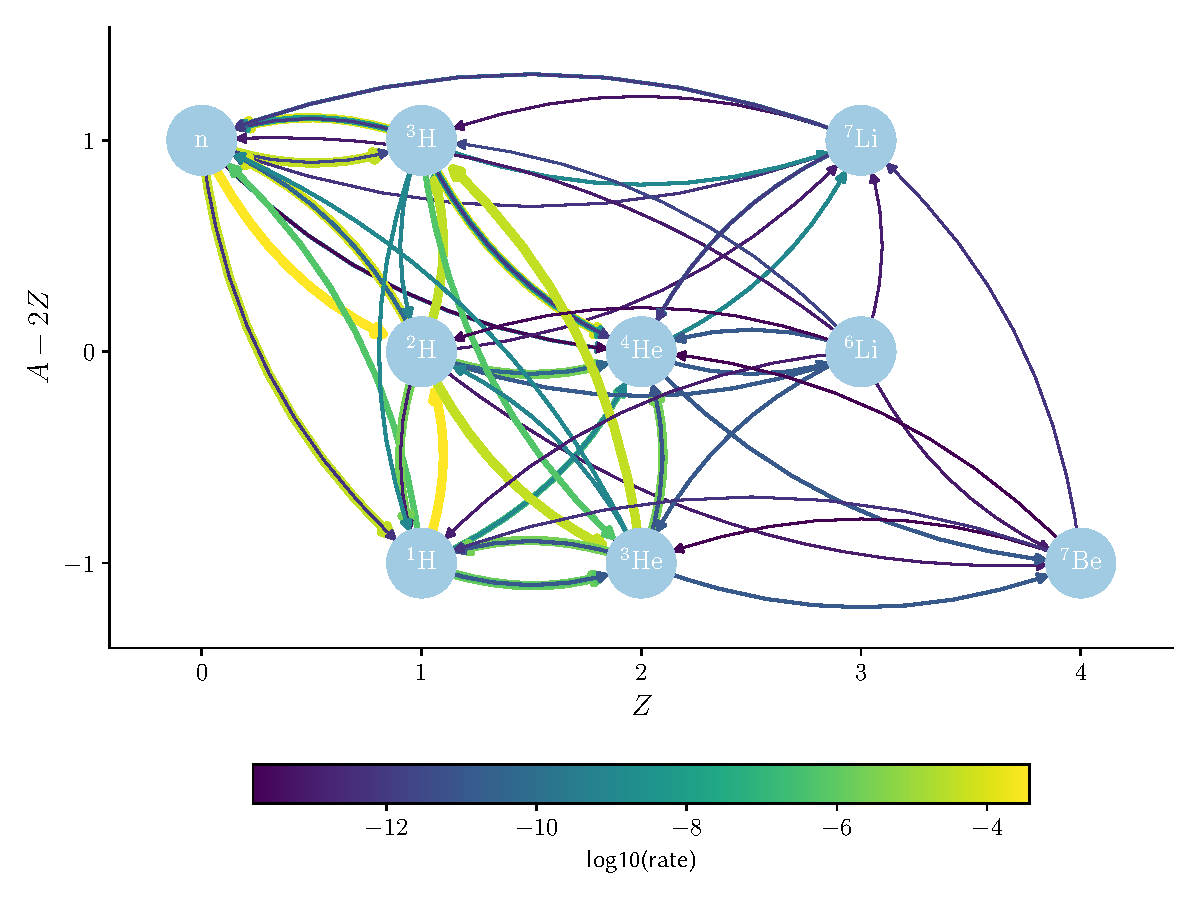
\includegraphics[height=10cm,trim={2cm 4.5cm 1cm 0},clip]{figures/smallnet5minutes.pdf}

    \vspace{1cm}

    \fontsize{16pt}{20pt}\selectfont
    \spread{Hans Br{\"u}ner Dein}\par
    \spread{201706079}\par

    \bigskip

    \fontsize{14pt}{18pt}\selectfont
    \spread{Master's Thesis in Physics}\par
    \spread{February 2024}\par
    %\bigskip
    \vfill

    Supervisors: Thomas Tram \& Steen Hannested\par
    % \href{http://pure.au.dk/portal/da/persons/id(XXX).html}{NAVN} \par

    \vfill

    \fontsize{12pt}{14.5pt}\selectfont
    \href{https://www.phys.au.dk/}{Department of Physics and Astronomy}\par
    \href{https://www.au.dk/}{Aarhus University}

  \end{adjustwidth*}

  % Colophon
  \newpage
  \begin{adjustwidth*}{\frontpagecorrection}{-\frontpagecorrection}
    \thispagestyle{empty}
    \strut\vfill
    {
      \setlength{\parindent}{0pt}
      \addtolength{\parskip}{.6em}

      \begin{center}
        \bfseries\sffamily Colophon
      \end{center}

      \small

      \textsl{\projecttitle}

      {--- \textsl{\projecttitledanish}}

      \smallskip

      Master's thesis by Hans Br{\"u}ner Dein. Written under supervision by Asc.Prof. Thomas Tram \& Prof. Steen Hannested
      Department of Physics and Astronomy, Aarhus University.

      Typeset by the author with \LaTeX{} and the \textsf{memoir} document class,
      using Linux Libertine and Linux Biolinum {\fontandleading}.

      Printed at Aarhus University
    }
  \end{adjustwidth*}
\end{titlingpage}


% ~~~~~~~~~~~~~~~~~~~~~~~~~~~~~~~~~~~~~~~~~~~~~~~~~~~~~~~~~~~~~~~~~~~~~~~~~~~~~
% Abstracts
% ~~~~~~~~~~~~~~~~~~~~~~~~~~~~~~~~~~~~~~~~~~~~~~~~~~~~~~~~~~~~~~~~~~~~~~~~~~~~~
\thispagestyle{chapter}

% ~~~~~~~~~~~~~~~~~
% Abstract: English
% ~~~~~~~~~~~~~~~~~
\begin{multiabstract}{Abstract (English)} 
\noindent The goal of this thesis is to present the development of a new BBN code APODORA (Adaptable Python interface Offering Determination Of Relic Abundances). APODORA is designed to be more flexible than existing codes, with an emphasis on the use of modern standardized computing methods. Derivations of the equations describing the time evolution of various components in the early universe are presented. These are implemented in a flexible IPython environment with the reaction network being created using interfaces from pynucastro\cite{pynucastro2}. The numerical uncertainty associated with every relevant input parameter of the code is systematically examined to ensure a high level of numerical precision. An in-depth comparison between APODORA and \textsc{AlterBBN} is performed, demonstrating equal or superior precision and speed. Finally, the resulting final abundances from APODORA are compared with multiple existing BNN codes as well as observational data.

\end{multiabstract}


% ~~~~~~~~~~~~~~~~~
% Abstract: Danish
% ~~~~~~~~~~~~~~~~~
\plainbreak{2}

% Switch to Danish
\selectlanguage{danish}
\begin{multiabstract}{Resumé (Dansk)}
\noindent Målet med dette speciale er at præsentere udviklingen af en ny BBN-kode APODORA, (Adaptable Python interface Offering Determination Of Relic Abundances). APODORA er skabt med henblik på at være mere fleksible end eksisterende løsninger, men særlig fokus på anvendelsen af moderne og standardiserende løsningsmetoder. Udledning af ligningerne som beskriver tidsudviklingen af det tidlige univers bestanddele bliver præsenteret. Dette er implementeret i et fleksibelt IPython miljø, hvortil reaktionsnetværket bliver skabt ved hjælp af brugerflader fra pakken pynucastro\cite{pynucastro2}. Den numeriske usikkerhed forbundet med hver relevant inputparameter i koden undersøges systematisk, for at sikre et højt niveau af numerisk præcision. Der udføres en dybdegående sammenligning mellem APODORA og \textsc{AlterBBN}, som påviser at både hastighed og præcision er lige så god, hvis ikke bedre. Til sidst sammenlignes forudsigelserne fra APODORA med andre BNN-koder samt observationer.

\end{multiabstract}

% Reset document language to English
\selectlanguage{english}

% List of fixme-notes -- REMEMBER TO REMOVE!
%  --> When removed, things will end on the correct pages
\listoffixmes

% Preface (Danish: Forord)
% [comment-out if not required]
%% ============================================================================
%%
%%  Speciale / Master's thesis
%%
%%  Author: FORNAVN EFTERNAVN
%%
%%  Preface
%% ============================================================================

%\chapter{Preface}
%\label{chap:preface}

%\centering Acknowledgments

\begin{multiabstract}{Acknowledgements} 
\noindent First and foremost, I would like to thank my friends and family for supporting and believing in me throughout the entirety of my time at IFA. For this thesis, I would like to thank my supervisor Thomas Tram, and unofficial co-supervisor Steen Hannested, for helping me along the way and ensuring I reached the goal in the end. I would also like to thank Erik Steenberg, Camilla Sørensen, Emil Birk, and Marta Jensen for proofreading the first and second draft of this thesis. In addition, I want to thank all the people at 1520-823, and in particular Christiane Rahbek, for providing company during the long days and nights of writing this thesis. I would also like to thank the pynucastro team for being very helpful in quickly fixing bugs and adding necessary features, with special thanks to Michael Zingale. 

Finally, I would like to thank my grandfather for igniting the passion for science, which has led me to this moment.

\end{multiabstract}
%This thesis concludes my Master's degree in/at .....


% Table of contents
\clearpage
\tableofcontents*

% Introduction (as an actual chapter, but *without* a number)
% [comment-out if not required]
%% ============================================================================
%%
%%  Speciale / Master's thesis
%%
%%  Author: FORNAVN EFTERNAVN
%%
%%  Introduction
%% ============================================================================

\chapter{Introduction}
\label{chap:intro}

Everything we see around us is made of atoms, which at their core contain a nucleus. Atomic nuclei are the fundamental building blocks that make up the stars, planets, and the humans that live on them. Understanding the creation of atomic nuclei is to understand the origin of the world itself. 


\subsection*{A Brief History of Early Nucleosynthesis}
When the universe was only a microsecond old, quarks coalesced to form the first protons and neutrons\cite{NASAUniversehistory}. Initially, there was an equal amount of neutrons and protons, but as the universe cooled, the slightly lighter protons became favored. The neutrons and protons remained in thermal equilibrium until the universe cooled to around $10^{10}$K, a second after the Big Bang. Here, the interaction between neutrinos and baryons becomes too weak to maintain thermodynamic equilibrium, freezing the ratio of neutrons and protons at one to five. The protons and neutrons can fuse to create deuterium, but these nuclei are short-lived as their low binding energy makes them vulnerable to destruction by the abundant high-energy photons. As these photons cool, the average lifetime of deuterium increases,
giving the deuterium nuclei more time to combine into much more stable helium nuclei. The rate of helium creation increases until it becomes great enough to rapidly convert all available neutrons into helium at approximately 200 seconds. Due to the delay caused by deuterium, the temperature and density of the universe will be too low to create any more than trace amounts of heavier elements. And so, a few minutes after it began, primordial nucleosynthesis ends. Barring radioactive decay, the abundance of the various elements will remain unchanged until the first stars appear $10^8$ years later\cite{klessen2023firststars}. 
The first computer code describing this process was created by Robert Wagoner in the late sixties\cite{Wagoner67}. Since then, many others have followed, with each implementation having its advantages and disadvantages.
\clearpage
\section{Objective} 
The objective of this thesis is to create a new state-of-the-art BBN code from first principles. To differentiate this code from existing implementations, it must fulfill these five requirements:

\begin{itemize}
    \item \textbf{Accessibility}: The code needs to run on any machine without the use of any proprietary software or special environments. %To achieve this, my code will require nothing but Python 3.0 and publicly available packages.
    \item \textbf{Accuracy}: The results must be consistent with those of contemporary BBN codes. Additionally, the results must be internally consistent with well-constrained numerical errors. 
    \item \textbf{Alacrity}: The code must be as fast as other contemporary BBN codes.
    \item \textbf{Agnostic reaction rates}: The code should use nuclear reaction rates from a single publicly available database to avoid any bias in rate selection.
    \item \textbf{Adaptability}: The code should be flexible and allow the investigation of various physical processes without changing the basic structure.
\end{itemize}

\section{Outline}

This thesis has three main parts:

\noindent First we will go over the physics required to describe the Big Bang nucleosynthesis. This will entail deriving every necessary relation from fundamental equations of cosmology, statistical physics, and thermodynamics. 

\noindent Next, we will review the numerical implementation of BBN. We start by covering the history and numerical difficulties associated with BBN calculations. The implementation of APODORA will then be briefly discussed, including the steps taken to overcome the aforementioned numerical difficulties.


\noindent Finally, we will look at the results. First, we will look at how APODORA can be used to get an overview of the various nuclear processes during BBN. Then, we will discuss the numerical accuracy of the code and how different parameters influence the precision. Ultimately, we compare with the results of other codes and observations.





\subsubsection{Terminology}

In the later sections of the thesis, predicted values for various nuclear abundances will be shown. For historical reasons, these are usually given as a molar faction relative to the abundance of hydrogen. That is to say, the number of nucleons contained in the particular isotope relative to the amount of free protons. ${}^4$He is an exception and is instead expressed as a fraction of total nucleons and denoted by $Y_p$. Though not entirely accurate, both of these molar fractions are often referred to as mass fractions. 

As BBN represents a crossover of nuclear physics and astronomy, temperature is interchangeably measured in MeV and Kelvin. Here, it is helpful to remember MeV$=11.6\times10^9 $K or simply MeV$\approx 10^{10}$K.


%\textcolor{orange}{Her skal nok tilføjes mere, afhængigt af hvilke termer DIG, korrekturlæserne ikke kender :)}


% ~~~~~~~~~~~~~~~~~~~~~~~~~~~~~~~
% Mainmatter (the actual content)
% ~~~~~~~~~~~~~~~~~~~~~~~~~~~~~~~
\mainmatter

% Here the chapters are organised in individual files, but in the same folder.
% Another option is to make one folder per chapter. This can e.g. be useful if
% each chapter contains many figures.

% Chapter 1
%% ============================================================================
%%
%%  Master's thesis
%% 
%%  Author: FORNAVN EFTERNAVN
%%
%%  Chapter 1: Coffee
%% ============================================================================

\chapter{BBN physics and cosmology}
\label{chap:theory}

This will be about the physics of BBN.

% ~~~~~~~~~~~~~~~~~~~~~~~~~~~~~~~~~~~~~~~~~~~~~~~~~~~~~~~~~~~~~~~~~~~~~~~~~~~~~
% SECTION
% ~~~~~~~~~~~~~~~~~~~~~~~~~~~~~~~~~~~~~~~~~~~~~~~~~~~~~~~~~~~~~~~~~~~~~~~~~~~~~
\section{cosmology}
\label{sec:cosmology}

citation test\textcite{kww}

\subsection{Electron/positron density and pressure}

\lipsum


% ~~~~~~~~~~
% SUBSECTION
% ~~~~~~~~~~
\subsection{Nuclear reactions}
\label{sec:nucleartheory}

Warning test\fxwarning{This is a warning!}

\lipsum


% Chapter 2
%% ============================================================================
%%
%%  Master's thesis
%%
%%  Author: FORNAVN EFTERNAVN
%%
%%  Chapter 2: Another topic....
%% ============================================================================

\chapter{BBN code}
\label{chap:BBNcode}

\section{History of BBN codes}
\label{sec:BBN_history}

The concept of Big Bang nucleosynthesis is almost as old as the Big Bang theory itself, with the with it first being proposed in the paper by \textcite{Gamov48}. This early model used neutron capture and subsequent beta decay as the mechanism for BBN, though its greatest problem was the inability to explain the unusually high abundance of oxygen and carbon in the present universe. And so, it was in large part supplanted by the new theory of stellar nucleosynthesis, as the main explanation for the origin of elements. 

During the next decades it became clear that stars could not be the only explanation for the present element abundances, and with the discovery of the CMB in 1965, new attention was brought to the early universe. 
Only a year later Peebles showed how simple BBN physics could be used to explain the high helium abundance, unaccounted for by stellar nucleosynthesis \cite{Peebles66}.

In the following years Wagoner created and refined the first proper BBN code, described in a series of defining papers\cite{Wagoner67}\cite{Wagoner69}\cite{Wagoner72}. With the legacy of this code still heavily influencing the way BBN calculations are performed today.

By the late 80s the Wagoner code was severely outdated. With multiple inefficiencies due to among other things, the fact that it was originally designed to run on punch cards. This inspired Lawrence Kawano to create the now ubiquitous NUC123, colloquially know as the Kawano code. Which set the gold Standard for all future BBN codes. 

In current day and age, there exists multiple publicly available BBN codes, and a countless number of private codes. The most well know of these are PArthENoPE spiritual successor to NUC123, AlterBBN, and PRIMAT.


\section{Structure of BBN codes}
\label{sec:BBN_structure}

The objective of any BBN code is to solve the system of differential equations described in chapter \ref{chap:theory}.

\subsection{Wagoner}
\label{sec:Wagoner}

\subsection{Kawano}
\label{sec:Kawano}

\subsection{Modern codes}
\label{sec:Modern_codes}
PArthENoPE, AlterBBN, PRIMAT


\subsection{AlterBBN}
\label{sec:AlterBBN}

AlterBBN is written in c and based on Kawano's NUC123. It maintains the same basic structure and integration method, though it uses natural units for everything but the reaction network. However, they define energy in GeV rather than MeV. What separates AlterBBN for other codes is that as the name implies, it allows the use of alternate cosmological models and parameters. Therefore, this code is especially well suited for testing the effects these alterations have on final abundances. Wot


% Chapter 1
\chapter{Output}
\label{chap:Results}
\begin{figure}[ht]
    %\centering
    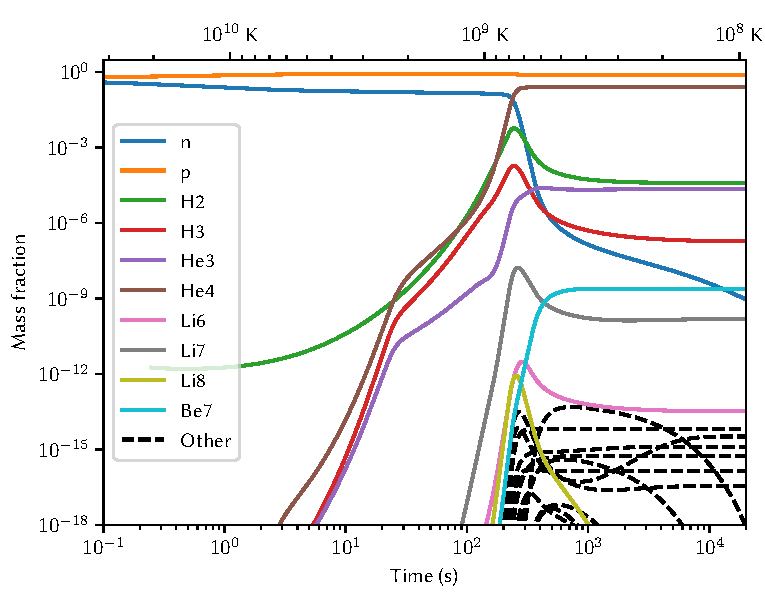
\includegraphics[width=5.1in]{figures/abundancelight.pdf}
    \caption{Time evolution of light nuclei abundance during BNN, with mass fraction technically being the close approximation $X_i=Y_i A_i$ }
    \label{fig:lightXevo}
\end{figure}
Running the code creates a complete overview of abundance evolution as shown on figure \ref{fig:lightXevo}. As expected neutrons protons and deuterium remain in equilibrium for the first few seconds. As the temperature decreases, deuterium abundances slowly increase quickly followed by tritium and both helium isotopes. %$2{}^2\text{H}\rightarrow {}^4\text{He}$ has a very small cross-section With ${}^4$H initially being produced primarily by ${}^3\text{H}+p\text{H}\rightarrow {}^4\text{He}$ and later by ${}^3\text{H}+{}^2\text{H}\rightarrow {}^4\text{He}+n$.
This continues until around 230 seconds, at which point the rate of ${}^4$He creation is finally great enough to have a significant impact on neutron abundance, which until then had remained almost unchanged since the $p\leftrightarrow n$ rates fell out of equilibrium. This leads to a rapid drop in neutron abundance creating a bottleneck on the production of deuterium and tritium. Without neutron capture to create more, the existing deuterium and tritium is converted to ${}^4$He via ${}^3\text{H}+{}^2\text{H}\rightarrow {}^4\text{He}+n$. Without these light nuclei lithium abundances also drop, as reactions such as ${}^4\text{He}+{}^3\text{H}\rightarrow {}^7\text{Li}$ become outmatched by the proton captures ${}^7\text{Li}+\text{p}\rightarrow 2{}^4\text{He}$ and ${}^6\text{Li}+\text{p}\rightarrow {}^7\text{Be}$. Conversely, Beryllium 7 is primarily destroyed via neutron capture ${}^7\text{Be}+\text{n}\rightarrow {}^7\text{Li}+\text{p}$, and therefore sees a rapid increase in abundance immediately after the drop in neutrons.
\begin{figure}[ht]
    %\centering
    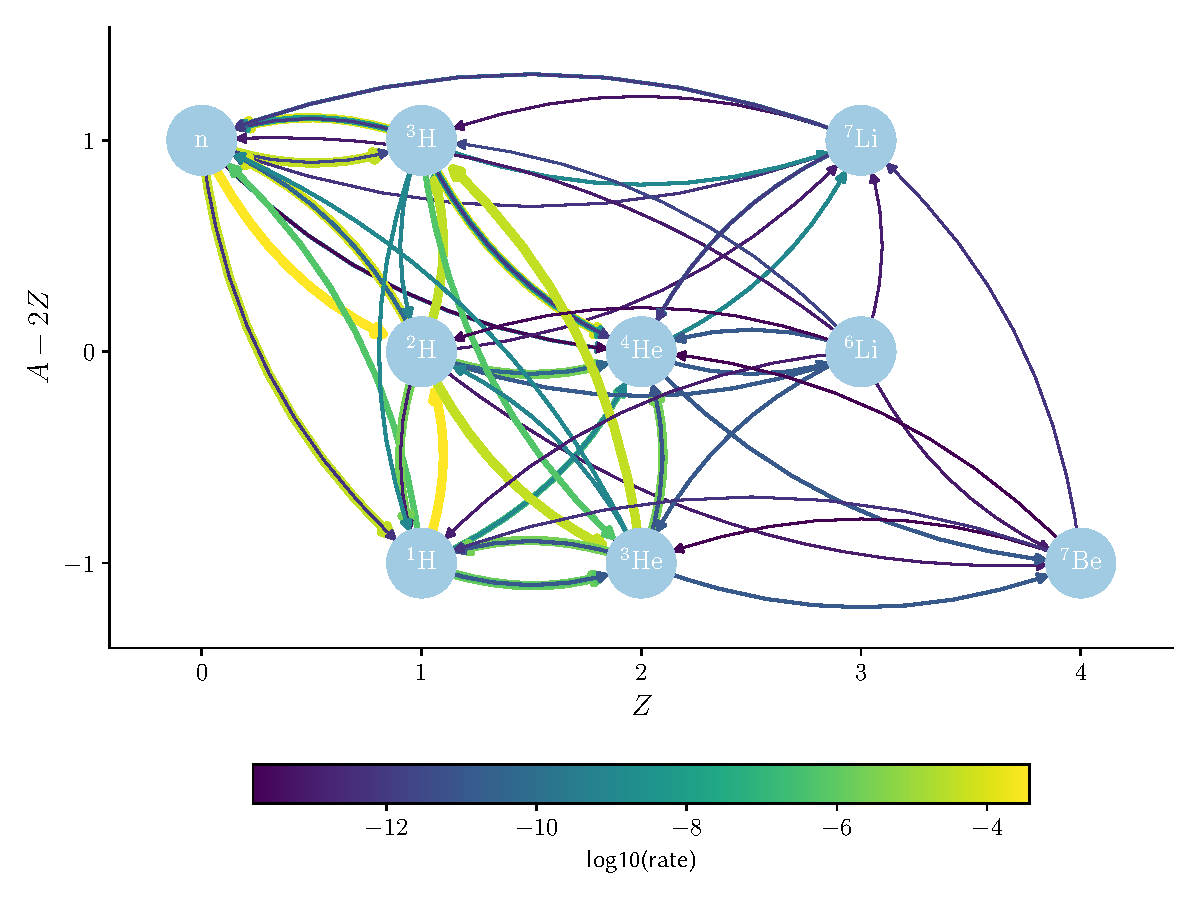
\includegraphics[width=5.1in]{figures/smallnet5minutes.pdf}
    \caption{Reaction rates 5 minutes after Big Bang at \num{7.6e8} K. Only including rates within 10 orders of magnitude of strongest. Each rate is represented by arrows from each reactant to each product}
    \label{fig:5minutenet}
\end{figure}

The relations of these reactions are illustrated in figure \ref{fig:5minutenet}. This snapshot is taken immediately after the aforementioned drop in neutron abundance with $Y_n=0.2\%$. Despite this $n+p\rightarrow d$ is still the strongest reaction rate, followed by rates creating ${}^3$He and ${}^3$H, simply due to the high abundance of these light nuclei. Though no particular reaction is exceptionally strong, a disproportionate amount of reactions produce rather than consume ${}^4$He. This should come as no surprise as ${}^4$He is the most tightly bound of all these nuclei. The only rates consuming helium are those producing heavier elements, ${}^4\text{He}+{}^3\text{H}\rightarrow {}^7\text{Li}$, ${}^4\text{He}+{}^3\text{He}\rightarrow {}^7\text{Be}$, and ${}^4\text{He}+{}^2\text{H}\rightarrow {}^6\text{Li}$. Yet these barely affect total helium abundance, and to an extent help create more ${}^4$He through subsequent reactions such as ${}^7\text{Li}+{}^2\text{H}\rightarrow 2 {}^4\text{He}+\text{n}$. 


\begin{figure}[ht]
    %\centering
    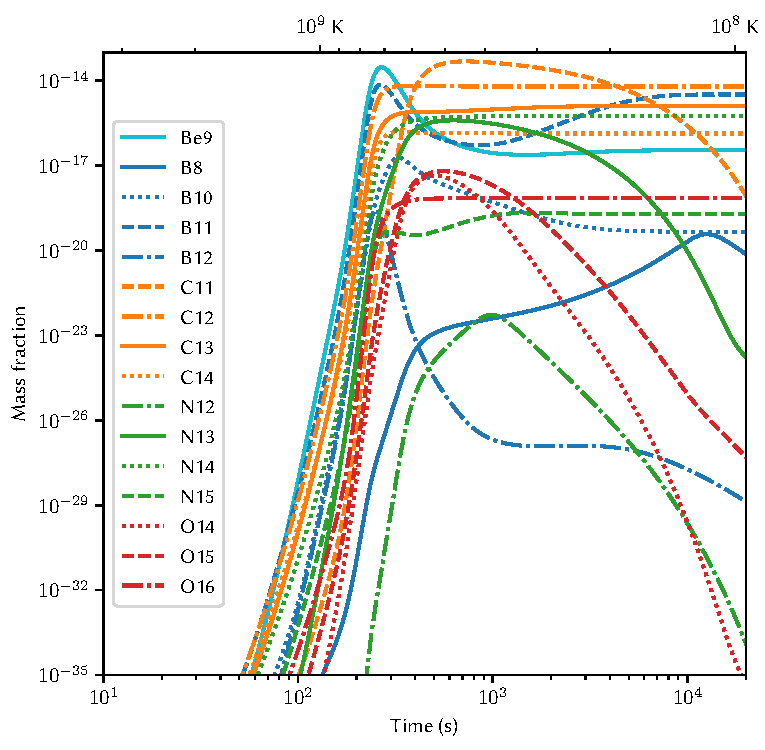
\includegraphics[width=5.1in]{figures/abundanceheavy.pdf}
    \caption{Time evolution of heavy nuclei abundance during BNN, with mass fraction technically being the close approximation $X_i=Y_i A_i$}
    \label{fig:heavyXevo}
\end{figure}

The most striking effect of the high ${}^4$He binding energy is the lack of stable nuclei with $A=8$, due 2 alpha particles being energetically favorable. Many nearby nuclei are also unstable creating a gap in the full reaction network, apparent on \ref{fig:bignet}. The next nucleus with greater binding energy per nucleon is ${}^{12}$C, which after BBN is also the most abundant of the heavy nuclei, as seen on figure \ref{fig:heavyXevo}. Bridging the gap between ${}^4$He and ${}^{12}$C is usually accomplished via the triple-alpha process $3{}^4\text{He}\rightarrow {}^{12}\text{C}$, which occurs in stars at temperatures above $10^8$K. The temperature during BBN is even higher than this, but compared to stellar interiors the density is much lower. At the previously mentioned 5 minute mark, the baryon density of the universe is only 10 grams per cubic meter, which is more than ten orders of magnitude lower than that of a helium burning stellar core. This completely stops the triple-alpha process, leaving the inefficient process of alpha capture on ${}^7$Li and later ${}^7$Be as the only options for creating heavier nuclei. This firstly creates ${}^{11}$B, which is through proton capture is responsible for the majority of ${}^{12}$C production. Unfortunately the resulting exited state ${}^{12}$C* predominately decays into three alpha particles, with the branching ratio of internal translation into the ground state being only \num{1.5e-4}. The same is true for neutron capture on ${}^{11}$C, though it also decays via proton emission  ${}^{12}\text{C}^\ast \rightarrow {}^{11}\text{B}+\text{p}$ and of course freely decays ${}^{11}\text{C}\rightarrow {}^{11}\text{B}$. From figure \ref{fig:heavyXevo} we also see an initial bump in ${}^9$Be abundance caused by the uniquely high cross-section of the reaction ${}^7\text{Li}+{}^3\text{H}\rightarrow {}^9\text{Be}+n$, but as tritium abundance drops most ${}^9$Be is destroyed by photofission $\gamma+{}^9\text{Be}\rightarrow 2{}^4\text{He}+n$.


\section{Precision}

Throughout the code there are several places where numerical accuracy must be balanced by the need for swift computation. As a baseline I aim for a relative precision on final abundances of $10^{-5}$ due to numerical uncertainty. This is much lower than the error introduced by the experimental determination of reaction rates, as well as that of astronomical observations of primordial abundances. 

\subsection{Tolerances}
For the integration itself I use the solve\_ivp method from scipy.integrate\cite{SciPy}. Here ensuring numerical accuracy is a simple matter of specifying the desired relative and absolute tolerances as optional parameters, which I have set as  rtol=1e-6 and atol=1e-80. The absolute tolerance might seem exorbitantly low, but this helps improve stability since some heavy nuclei can cause detrimental transients if not tracked accurately at even minute abundances. However, for the tests this section I use rtol=1e-8, to ensure any inaccuracy is caused be whatever parameter is being tested.


\subsection{Electron energy}
Most calculations for the background have nice analytical expressions that can be computed with arbitrary precision. The electron energy density is the main exception, as it is given by an infinite sum \eqref{eq:rhoelectron} of which a finite number of terms must be calculated. Electrons annihilate very early, so any error in the energy density will only affect the $p\leftrightharpoons n$ rate. This will lead to a small change in neutron abundance, which results in a similar (within one order of magnitude) relative change in the abundance of all subsequent nuclei. 
Testing shows that small changes to the energy density, cause a change in neutron abundance of roughly the same relative magnitude if not slightly lower. So to achieve the requested accuracy in abundance, I will also aim for a $10^{-5}$ relative error in total energy density. 
\begin{figure}[ht]
    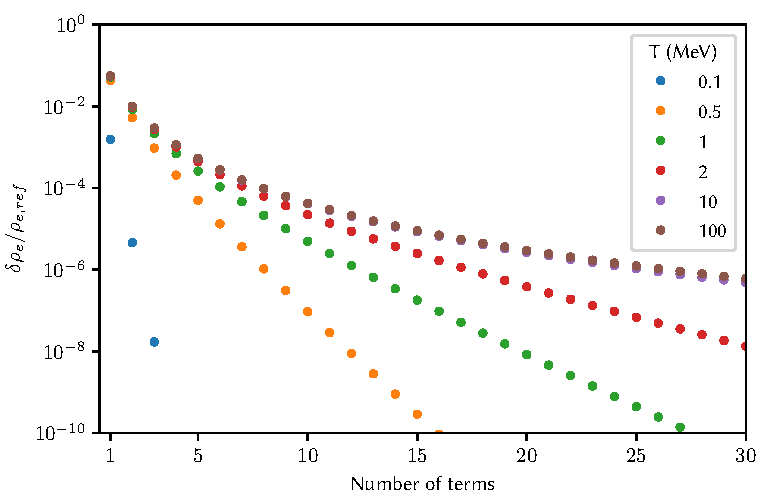
\includegraphics[width=5.1in]{figures/Besselaccuracy.pdf}
    \caption{Normalized absolute deviation of electron energy density from the reference energy as a function of included terms in \eqref{eq:rhoelectron}. The reference energy density has been determined by computing the first 10000 terms}
    \label{fig:Besselaccuracy}
\end{figure}

Figure \ref{fig:Besselaccuracy} shows the deviation from the reference energy at select temperatures before and during e$^-$ e$^+$ annihilation. For low temperatures the sum converges quickly, which should come as no surprise as the series in \eqref{eq:electronseries}, converges more rapidly as $e^{-(E\pm\mu)/T}$ approaches 0. At high temperatures the sum converges at a much slower rate, but it still achieves sufficient accuracy with only 20 terms, which is the number I will use moving forward.

\subsection{Interpolation}
\label{sec:interpolation}
For the interpolation on background variables an appropriate number of points must be selected. These points are spaced uniformly in log(t). Tests show that $10^4$ points is sufficient to achieve the required accuracy in final abundances. However, a low number of points cause the small discontinuities in the derivatives of temperature and scale factor. Due to the stiffness of the system this leads to instabilities, which have a major impact on the runtime. At the required resolution of $10^4$ the integration routine has to make twice as many call to the RHS, compared to smoother integration. At $2\times 10^5$ points the interpolations is smooth enough as to not cause issues for integration.


\subsection{Network timings}
\label{sec:networktiming}
As  mentioned in section \ref{sec:pna}, we cannot calculate the abundance of all nuclei from the beginning, and have to add them gradually as the y become relevant. To find this point we can plot the deviation in final abundance as a function of the time at which we switch between networks.
\subsubsection{Full network}
We start by looking at the full network shown on figure \ref{fig:bignettime}, which has three distinct points. As long as the heavy nuclei are added before 2 minutes corresponding to $T>10^9$K they have time to reach the same abundance as they would if they were added earlier. Adding them later will delay the initial production, which will slowly lower the resulting final abundance. They will however still reach approximately the same final abundance until the late stages of BBN at around 7 minutes. Here the temperature will be to low for their formation, resulting in an increase in Lithium and Beryllium, as these are no longer consumed to produce heavy nuclei. The reaction involving ${}^{11}$C however come into effect much later than most other reactions and remain relevant even an hour after BBN. If ${}^{11}$C is added after this point, it will never achieve a significant final abundance, leading to a drop in its indirect daughter nuclei ${}^{9}$Be and ${}^{6}$Li. 
\begin{figure}[ht]
    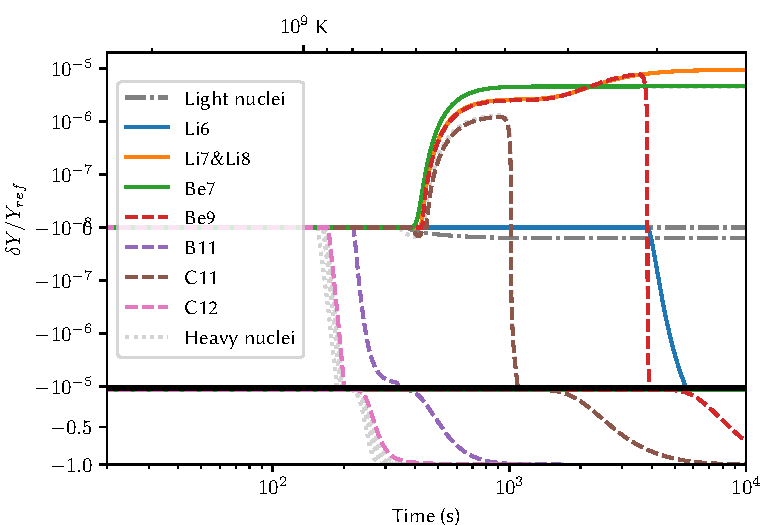
\includegraphics[width=5.1in]{figures/Bignettime.pdf}
    \caption{Relative deviation on final abundances based on the time from which heavy nuclei are included in the reaction network. To display both positive and negative changes, relative deviations $ <10^{-8}$ are excluded. The bottom shows negative deviation on a linear scale}
    \label{fig:bignettime}
\end{figure}

The result of this test shows that for standard BBN heavy nuclei don't actually need to be included at all, if one is only interested in abundances of light nuclei. For completeness, I will choose to include these nuclei anyway starting at $T>10^9$K. 

\subsubsection{Light network}

From figure \ref{fig:midnettime} we see that delaying the calculation of nuclear abundances, initially cause an increase abundance of protons and the proton dominated nuclei ${}^3$He and ${}^8$B, with all other abundances dropping. This is due to early nuclear reactions trapping neutrons in the cores light nuclei such as ${}^4$He and ${}^2$H, preventing their free decay into protons. However, since the vast majority of neutrons are still unbound, this effect will be insignificant until large light nuclei abundances are attained. Therefore, we actually don't need to calculate early abundances to get precise estimates of the final abundance. 

\begin{figure}[ht]
    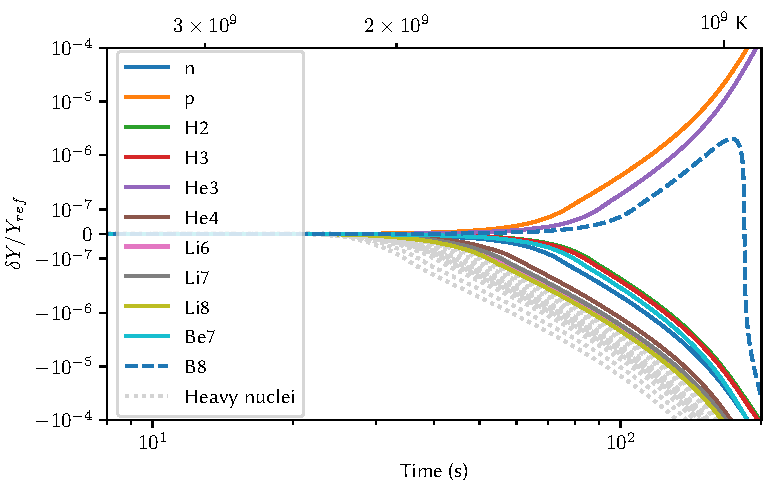
\includegraphics[width=5.1in]{figures/midnettime.pdf}
    \caption{Relative deviation on final abundances based on the time from which light nuclei are added to the reaction network. Plot is linear in the region $\pm 10^{-7}$ and logarithmic outside}
    \label{fig:midnettime}
\end{figure}
Not having to solve the reaction network at high temperatures makes the system much less stiff, potentially allowing future BBN codes to use less complex integrations routines than those used by this and older codes. Unfortunately starting abundance calculations presents a major issue due to the initial conditions. When starting light abundance calculation at early times $t<10$s, we can determine the initial abundances by setting the RHS to 0 as described in section \ref{sec:structure}. But at later times reactions destroying ${}^4$He drop off, with ${}^4$He abundances instead being kept in check by the lack of deuterium. As the system is no longer in exact NSE, any method for determining initial condition which assume a steady state solution will fail. Given enough time all neutrons will be converted to ${}^4$He, and the estimated initial conditions reflect this by vastly overestimating ${}^4$He abundances. To get around this and produce figure \ref{fig:midnettime}, I instead had to set all initial abundances to 0 when initiating the light network after 3 seconds. This workaround eliminates the problem, but creates another in the form of transients create as abundances go from 0 to their appropriate value. Since the system of equations is less stiff at these late times the transients won't break the integration. But dealing with these transients takes just as long as the time required for just tracking abundances at early times. 


\subsubsection{$p\leftrightharpoons n$ network}
Unlike the heavier nuclei the at which we start calculating neutrons and protons abundances have a very abrupt and significant impact on final abundances. As long as they are still in thermal equilibrium when we begin calculations, the final abundance will be the same. Conversely, if we start after they begin to fall out of thermal equilibrium, all final abundances will be radically different. From figure \ref{fig:npnettime} it's clear that this occurs at around 100 ms or \num{3e10}K, and as long as we initiate $p\leftrightharpoons n$ before this we get precise results. This also justifies the use of 27e9 K as the initial temperature, which is the point used by among others Wagoner, Kawano, and AlterBBN.
\begin{figure}[ht]
    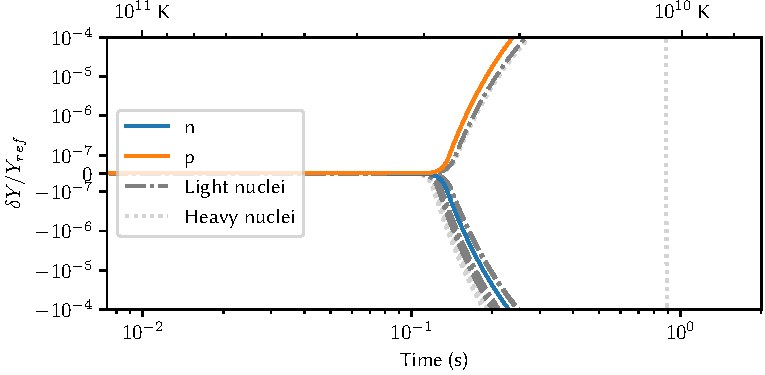
\includegraphics[width=5.1in]{figures/npnettime.pdf}
    \caption{Relative deviation of final abundances based on the initial time of BBN calculations. Plot is linear in the region $\pm 10^{-7}$ and logarithmic outside}
    \label{fig:npnettime}
\end{figure}



\subsection{Neutrino decoupling}

The main source of inaccuracy in this code is the assumption of complete neutrino decoupling. This assumption is reasonable as the only net transfer of energy between different particles is annihilation of electrons and positrons, which begins at around 1 MeV as shown on figure \ref{fig:rhoegammaT}. This is long after the neutrinos have decoupled, and therefore the energy is transferred to the photons, which are heated relative to the neutrinos by the well known factor $\sqrt[3]{11/4}$. There is however a small transfer of energy before the neutrinos completely decouple from the other particles. The result of this is a small increase in neutrino temperature relative to photon temperature of less than 1\% \cite{Hannestad:1995rs}. As both neutrinos and photons are ultrarelativistic, this change is inconsequential to the time evolution of the early universe, and should intuitively not have a significant impact on final abundances. This is however not the case, as is apparent from figure \ref{fig:initime}. The reason for this is that the higher photon temperature caused by instantaneous decoupling, effectively delays the onset of nucleosynthesis, since the baryons take longer to cool sufficiently. This has two main effects, the first being slightly lower baryon density at any given temperature, and the second that the universe will remain in any given temperature range for longer. Additionally, neutrino decoupling also affects the $p\leftrightharpoons n$ reactions directly, as these rely on both exact temperature and non-thermal energy distribution of the neutrinos. When assuming complete neutrino decoupling, these effects lowers the abundance of ${}^4$He by 0.05\%, ${}^3$He by 0.1\%, and deuterium by 0.5\%, and increase ${}^7$Be by 0.5\%, (PRIMAT table V\cite{PRIMAT}). 


Since my implementation uses estimated $p\leftrightharpoons n$ rates which do take into account incomplete neutrino decoupling, my results are primarily affected by the delaying of nucleosynthesis, caused by the inaccurate $T_\nu/T\gamma$ ratio. To reduce the deviation in $T_\nu/T\gamma$ ratio, we can decouple the neutrinos as close as possible to the point at which they actually decouple. This still assumes an instant rather than gradual decoupling, but nonetheless improves predicted abundances. The point at which neutrinos decouple obviously coincide with the freezeout of $p\leftrightharpoons n$ reactions, and as shown on \ref{fig:npnettime}, we can safely begin both background and network integration at 27 GK corresponding to 2.3 MeV. 
\begin{table}[ht]
    \begin{tabular}{l|llllll}
        & $Y_p \times 10$ & \hspace{-0.34em}$^{2}$H$ \times 10^{5}$ & \hspace{-0.34em}$^{3}$He$ \times 10^{5}$ & \hspace{-0.34em}$^{7}$Li $ \times 10^{10}$& \hspace{-0.34em}$^{6}$Li $ \times 10^{15}$& \hspace{-0.34em}$^{7}$Be $ \times 10^{10}$\\ \hline
    100 MeV & 2.470            & 2.532 & 1.040 & 4.712 & 7.503 & 4.411     \\ \hline
    2.3 MeV  & 2.472            & 2.536 & 1.040 & 4.706 & 7.523 & 4.404   \\ \hline
    Deviation & 0.07\%           & 0.15\% & 0.04\% & -0.15\% & 0.25\% & -0.18\%      
    \end{tabular}
    \caption{Comparison of final abundances for instant decoupling at 2.3 and 10 MeV, with all abundances except ${}^4$He ($Y_p$) being normalized to H abundance. ${}^3$He and ${}^7$Li including contribution from eventual decay of ${}^3$H and ${}^7$Be}
    \label{tab:earlylatedecoup}
\end{table}

From table \ref{tab:earlylatedecoup} we clearly see the impact of neutrino decoupling. Compared to the expected changes determined by PRIMAT\cite{PRIMAT}, we see an increased impact on ${}^4$He and a reduced impact on ${}^7$Be and ${}^3$He. This can mostly be explained by the $p\leftrightharpoons n$ reactions not being directly impacted in my implementation. The direct effect on $p\leftrightharpoons n$ increases the neutron abundance subsequently the abundance of all other nuclei, counteracting the effects on everything but ${}^7$Be, as well as ${}^3$He since its abundance actually increases as neutron abundance drops.%The direct effect only changes the neutron proton ratio, which partially cancels the changes introduced by the delay of nucleosynthesis, particularly in ${}^4$He abundance. Therefore, the theoretical systematic error in ${}^4$He is slightly higher, which we will explore further in section \ref{sec:Altercompare}.
\begin{figure}[ht]
    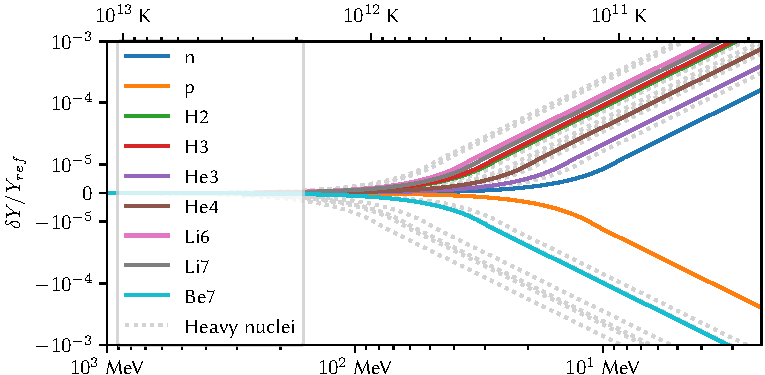
\includegraphics[width=5.1in]{figures/initime.pdf}
    \caption{Relative deviation on final abundances based on the initial time for background calculations. By construction the initial time coincides with the time of neutrino decoupling}
    \label{fig:initime}
\end{figure}

Though the errors associated neutrino decoupling are much greater than the achieved numerical error of less than $10^{-5}$, they are still acceptable, since they are completely inconsequential next to the uncertainty associated with reactions rates, as will become apparent in the following section.


\section{Comparison with AlterBBN}
\label{sec:Altercompare}
To compare the results of this code to that of other contemporary BBN codes, I have chosen AlterBBN. The main reason for this is that my code is written in Python with much of the heavy computation being done directly in C. This makes it easier to interface with the C based AlterBBN than PArthENoPE or PRIMAT, which as previously mentioned are written in FORTRAN and Mathematica. 
\begin{table}[ht]
    \begin{tabular}{l|llllll}
        & $Y_p \times 10$ & \hspace{-0.34em}$^{2}$H$ \times 10^{5}$ & \hspace{-0.34em}$^{3}$He$ \times 10^{5}$ & \hspace{-0.34em}$^{7}$Li $ \times 10^{10}$& \hspace{-0.34em}$^{6}$Li $ \times 10^{14}$& \hspace{-0.34em}$^{7}$Be $ \times 10^{10}$\\ \hline
    This work & 2.472            & 2.536 & 1.040 & 4.706 & 0.752 & 4.404   \\ \hline
    AlterBBN & 2.474            & 2.467 & 1.034 & 5.363 & 1.087 & 5.075   \\ %\hline
    $\quad +/-$ & 0.003           & 0.038 & 0.016 & 0.352 & 1.085 & 0.343      
    \end{tabular}
    \caption{Abundances from this work and AlterBBN, with all abundances except ${}^4$He ($Y_p$) being normalized to the H abundance. ${}^3$He and ${}^7$Li including contribution from eventual decay of ${}^3$H and ${}^7$Be. Quoted uncertainties are those determined by AlterBBN}
    \label{tab:shortAlterabun}
\end{table}


Comparing the final abundances predicted by this code and AlterBBN we see major discrepancies. Most of these are within the uncertainties calculated by AlterBBN based on the uncertainty of the reaction rates. ${}^7$Be and subsequently ${}^7$Li deviate by more than twice what is predicted, and the same is true for deuterium. To discover the cause of this we can do a 1 to 1 comparison of the time evolution of the universe according to this work and AlterBBN. Here we use the exact same initial conditions of $T=27\times10^9$K, $\eta=6.1$e-$10$ and $\tau_n=880.2$s, remembering to correct for the inaccurate initial time in AlterBBN as explained in section \ref{sec:t_ini}.

\subsection{Background}
To rule out cosmological differences, we can compare the predicted background parameters from AlterBBN and this code, displayed on figure \ref{fig:comparetemp}. Unsurprisingly after the common initial temperature of 27GK, AlterBBN sees a relative increase in neutrino temperature due to incomplete neutrino decoupling, with photon temperature initially decreasing slower due to sharing temperature with the electrons. Later there is a small additional drop in photon temperature coinciding with the onset of primary nucleosynthesis. This can be explained by AlterBBN taking into account the effect of nucleosynthesis on photon temperature, due to the energy release of nucleosynthesis. However, the observed effect is unphysical and must be due to numerical errors, since the energy release is nowhere near the amount required for an impact on photon temperature of this size, and additionally it should serve to increase, rather than decrease the photon temperature. Lastly, there is a relative decrease of the AlterBBN neutrino temperature at late times. This is due to AlterBBN taking into account both baryon and dark matter energy density, which I have omitted since it clearly doesn't have a significant impact during the era of BBN.
\begin{figure}[ht]
    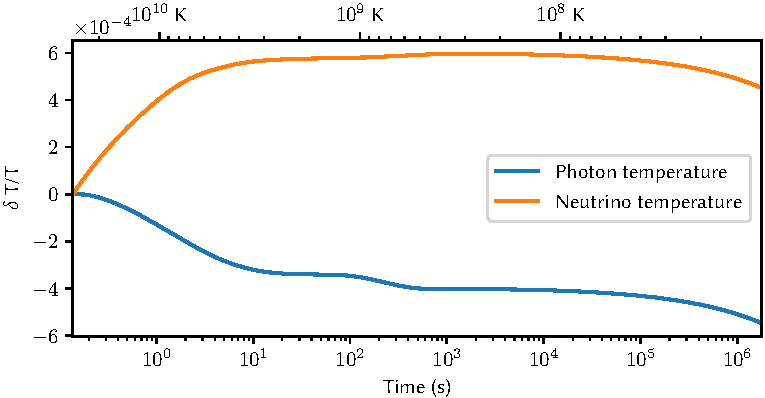
\includegraphics[width=5.1in]{figures/comparetemp.pdf}
    \caption{Relative deviation of temperatures as calculated by this code and AlterBBN. Positive values signify higher AlterBBN temperatures compared to this code}
    \label{fig:comparetemp}
\end{figure}

To see the impact of these background differences we can integrate the reaction network using the background parameters from AlterBBN. At its highest precision setting AlterBBN takes 64421 discreet time steps, which based the test in section \ref{sec:interpolation} is sufficient to achieve high accuracy with the existing interpolation routine. AlterBBN does however not directly track the scale factor, so we must instead track the baryon density using the neutrino temperature. Since the tabulated $p\leftrightharpoons n$ rates used in this network only depend on temperature, we don't need to know the exact value of $n_b$ before the other reactions become relevant at around 100 seconds, (figure \ref{fig:midnettime}). At this time neutrinos have actually decoupled completely, and therefore the relation $T_\nu \propto a^{-1}$ holds exactly. This allows the baryon number density to be determined by $n_b= C \cdot T_\nu^3$ with the constant $C$ being set by requiring $\eta=6.1$e-$10$ at late times.
\begin{table}[ht]
    \begin{tabular}{l|llllll}
               & $Y_p \times 10$ & \hspace{-0.34em}$^{2}$H$ \times 10^{5}$ & \hspace{-0.34em}$^{3}$He$ \times 10^{5}$ & \hspace{-0.34em}$^{7}$Li $ \times 10^{10}$& \hspace{-0.34em}$^{6}$Li $ \times 10^{14}$& \hspace{-0.34em}$^{7}$Be $ \times 10^{10}$\\ \hline
    100 MeV & 2.470            & 2.532 & 1.040 & 4.712 & 0.750 & 4.411     \\ \hline
    2.3 MeV  & 2.472            & 2.536 & 1.040 & 4.706 & 0.752 & 4.404    \\ \hline
    \begin{tabular}[c]{@{}l@{}}This work using \\ AlterBBN $T_\gamma$ \& $T_\nu$ \end{tabular} & 2.473            & 2.540 & 1.041 & 4.699 & 0.754 & 4.398   \\ \hline
    AlterBBN & 2.474            & 2.467 & 1.034 & 5.363 & 1.087 & 5.075   \\ %\hline
    $\quad +/-$ & 0.003           & 0.038 & 0.016 & 0.352 & 1.085 & 0.343     
    \end{tabular}
    \caption{Comparison of final abundances for various background parameters. Showing results of this network using early and late instant neutrino decoupling, as well as the AlterBBN background which accounts for incomplete decoupling. The last row shows result from the AlterBBN background using their own abundance calculations}
    \label{tab:longAlterabun}
\end{table}

The result of using the background parameters of AlterBBN are displayed on Table \ref{tab:longAlterabun}. Though somewhat obscured by the lack of significant digits, relative change caused by using the AlterBBN background is equal to 90\% of the change caused by changing the timing of instant neutrino decoupling. This is due to the increase in $T_\nu/T_\gamma$ predicted by full incomplete decoupling, being 1.9 times greater than what is achieved by simply delaying instant decoupling. ${}^4$He however only increases by 68\% of that caused by delayed decoupling. This is due to ${}^4$He being governed by the $p\leftrightharpoons n$ reactions, which take place while $T_\nu/T_\gamma$ is still increasing. This supports the previous assumption, that the only major difference between the cosmological calculation of AlterBBN and this code, is their inclusion of incomplete neutrino decoupling.

\subsection{Reaction network}

Since the difference in background introduces minimal abundance corrections, the discrepancy between the AlterBBN results and mine must unsurprisingly be due to differences in the reaction network. To see where these differences are we can plot the relative difference between abundances as they evolve during BBN, displayed on figure \ref{fig:AlterBBNdeltaY}. 
\begin{figure}[ht]
    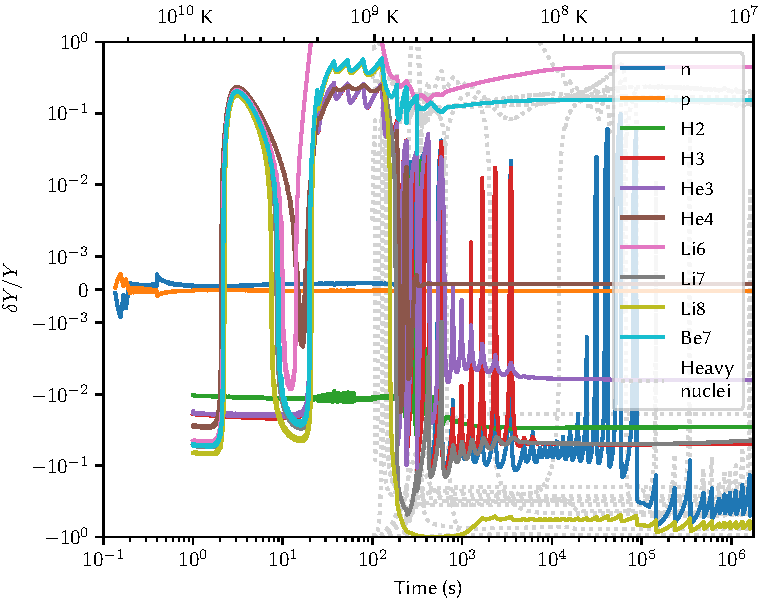
\includegraphics[width=5.1in]{figures/AlterBBNdeltaY.pdf}
    \caption{Relative deviation on abundances between this code and AlterBBN, during the various stages of BBN. To rule out cosmological differences, the AlterBBN background parameters are used for both calculations. Plot is linear in the region $\pm 10^{-3}$ and logarithmic outside}
    \label{fig:AlterBBNdeltaY}
\end{figure}
Staring with the lightest nuclei, we see the small difference in neutron proton ratio, and how this despite everything else, winds up resulting in an almost identical difference in $Y_p$. However, the most striking feature are the periodic spikes in relative abundance, affecting almost every single nuclei. This jaggedness originates in AlterBBN, and is caused by their implementation of certain reaction rates. As described in section \ref{sec:pna}, I use smooth fits of experimental data to obtain appropriate values for the reaction rates at any temperature. With every one of these rates stemming from the most recent snapshot of the REACLIB database\cite{REACLIB} available in pynucastro\cite{pynucastro2}. AlterBBN on the other hand uses a manually curated list of reaction rates, with a myriad of different sources and implementations. A few of these rates are tabulated, and to obtain values between the tabulated temperature steps, AlterBBN simply uses nearest neighbor interpolation. This is hard coded as a series of consecutive else/if statements, which return the value of the reaction rate in discreet steps according to the nearest tabulated value. The spikes happen whenever these rates assume a new value. As an example AlterBBN uses a tabulated ${}^2\text{H}+p\rightarrow {}^3\text{He}$ rate from \textcite{Coc_et_al_2015}, which is responsible for the small early spikes in ${}^3\text{He}$, and other nuclei that depend on its abundance. This can be confirmed by noting that the early spikes peak at 1.875, 1.625, 1.375, and 1.125 GK, which happen to be the exact midpoints between the tabulated values which are at 2, 1.75, 1.50, 1.25, and 1 GK. 

Another notable difference is the relative increase and subsequent drop in ${}^4\text{He}$ abundances, which takes place between 2 and 20 seconds. This is caused by the ${}^3\text{He}+n\rightarrow {}^4\text{He}$ rate. Here AlterBBN uses a linear approximation for the rate, which stems from the original Wagoner code\cite{Wagoner69}. Though inaccurate, this doesn't actually have a significant impact on final abundances since the reaction only dominates ${}^4\text{He}$ production at very early times. 





This leaves the main outliers, namely ${}^7\text{Li}$ and thereby ${}^7\text{Be}$. The primary reactions responsible for creating and destroying ${}^7\text{Li}$ are ${}^3\text{H}+{}^4\text{He}\rightarrow {}^7\text{Li}$ and ${}^7\text{Li} + p\rightarrow 2{}^4\text{He}$, with ${}^7\text{Be}$ being governed by ${}^3\text{He}+{}^4\text{He}\rightarrow {}^7\text{Be}$ and ${}^7\text{Be} + n\rightarrow {}^7\text{Li} + p$. Compared to these, all other reactions are completely insignificant, which can be seen on \cref{fig:Be7destruct,fig:Be7create,fig:Li7destruct,fig:Li7create}. Since AlterBBN and my network use different rates for each one of these reactions, 


For each of these four reactions a different rate is used by . 

\subsubsection{Modifying the Network with AlterBBN rates}
Due to the modular nature of my reaction network it is quite easy to simply swap the relevant reaction rates for those used by AlterBBN. Using the four ${}^7\text{Li}$ and ${}^7\text{Be}$ rates from AlterBBN as well as the previously mentioned ${}^3\text{He}+n\rightarrow {}^4\text{He}$ rate, a new set of final abundances can be obtained, \cref{tab:Alterratesabun}. 
\begin{table}[ht]
    \begin{tabular}{l|llllll}
               & $Y_p \times 10$ & \hspace{-0.34em}$^{2}$H$ \times 10^{5}$ & \hspace{-0.34em}$^{3}$He$ \times 10^{5}$ & \hspace{-0.34em}$^{7}$Li $ \times 10^{10}$& \hspace{-0.34em}$^{6}$Li $ \times 10^{14}$& \hspace{-0.34em}$^{7}$Be $ \times 10^{10}$\\ \hline
    Default rates  & 2.473    & 2.540 & 1.041 & 4.699 & 0.754 & 4.398    \\ \hline
    \begin{tabular}[c]{@{}l@{}}Rates from  \\ AlterBBN \end{tabular} & 2.473    & 2.540 & 1.041 & 5.133 & 0.754 & 4.837    \\ \hline
    AlterBBN & 2.474            & 2.467 & 1.034 & 5.363 & 1.087 & 5.075   \\ %\hline
    $\quad +/-$ & 0.003           & 0.038 & 0.016 & 0.352 & 1.085 & 0.343     
    \end{tabular}
    \caption{Final abundances for the default network, the network using select AlterBBN rates, and the results from AlterBBN}
    \label{tab:Alterratesabun}
\end{table}
As expected only the abundances of ${}^7\text{Li}$ and ${}^7\text{Be}$ are affected, since the total abundances of light nuclei involved in the four reactions are much higher. 
Though the modified rates bring ${}^7\text{Li}$ and ${}^7\text{Be}$ abundances within the estimated uncertainty of AlterBBN, they still deviate significantly. To explain this figure \ref{fig:AlterBBNdeltaY} can be recreated using the modified reaction network. 


Furthermore, the "new" ${}^3\text{He}+n\rightarrow {}^4\text{He}$ rate doesn't affect the final abundances. 


The abundances still deviate from that of AlterBBN, which is 


Using the major ${}^7\text{Li}$ and ${}^7\text{Be}$ rates from AlterBBN, we get updated final abundance


\begin{figure}[ht]
    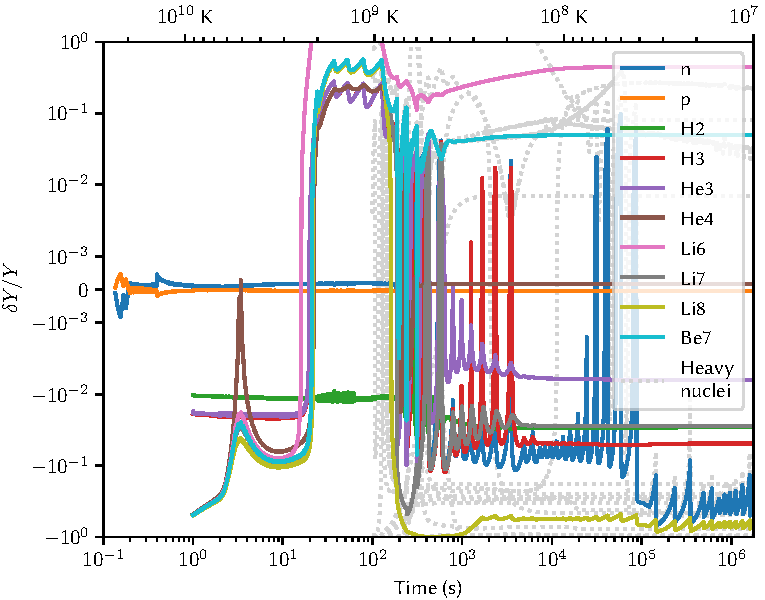
\includegraphics[width=5.1in]{figures/AlterratesBBNdeltaY.pdf}
    \caption{Same as \cref{fig:AlterBBNdeltaY}, but with the network using the same rates as AlterBBN for the reactions ${}^3\text{He}+n\rightarrow {}^4\text{He}$, ${}^7\text{Li}$ are ${}^3\text{H}+{}^4\text{He}\rightarrow {}^7\text{Li}$, ${}^7\text{Li} + p\rightarrow 2{}^4\text{He}$, ${}^3\text{He}+{}^4\text{He}\rightarrow {}^7\text{Be}$, and ${}^7\text{Be} + n\rightarrow {}^7\text{Li} + p$}
    \label{fig:AlterratesBBNdeltaY}
\end{figure}




I recreate figure \ref{fig:AlterBBNdeltaY} resulting in figure \ref{fig:AlterratesBBNdeltaY}. Looking at the early abundances we confirm that the initial difference in light nuclei abundance was indeed caused by the ${}^3\text{He}+n\rightarrow {}^4\text{He}$ rate. For the 



Comparing the swapping out the 




AlterBBN uses a different rate for each of these which 




\section{Final abundances}



\section{Nuclear solutions to the Lithium problem?}



% ~~~~~~~~~~~~
% Bibliography
% ~~~~~~~~~~~~
\clearpage

% Change the sorting of references to NAME-YEAR-TITLE (see preamble for details) change to Ynt because that works
\begin{refcontext}[sorting=ynt]
  % Standard bibliography
  \raggedyright[4em] \printbibliography
  % With custom title (activate in preamble)
  % \raggedyright[4em] \printbibliography[heading=memoirbib]
\end{refcontext}


% ~~~~~~~~~~
% Appendices
% ~~~~~~~~~~
\appendix
\chapter{Additional plots}
\label{chap:more_plots}

\begin{figure}[ht]
    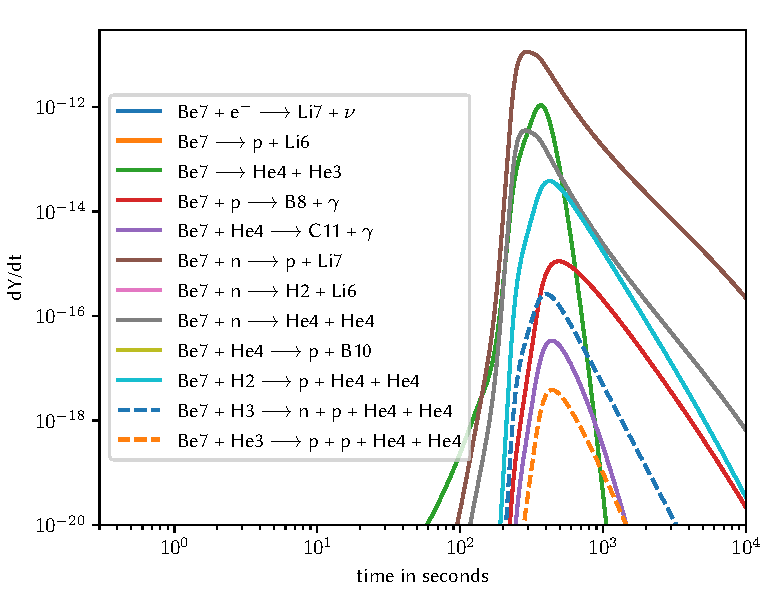
\includegraphics[width=5.1in]{figures/app/Be7destruct.pdf}
    \caption{Strength of different ${}^7$ Be destruction rates}
    \label{fig:Be7destruct}
\end{figure}

\begin{figure}[ht]
    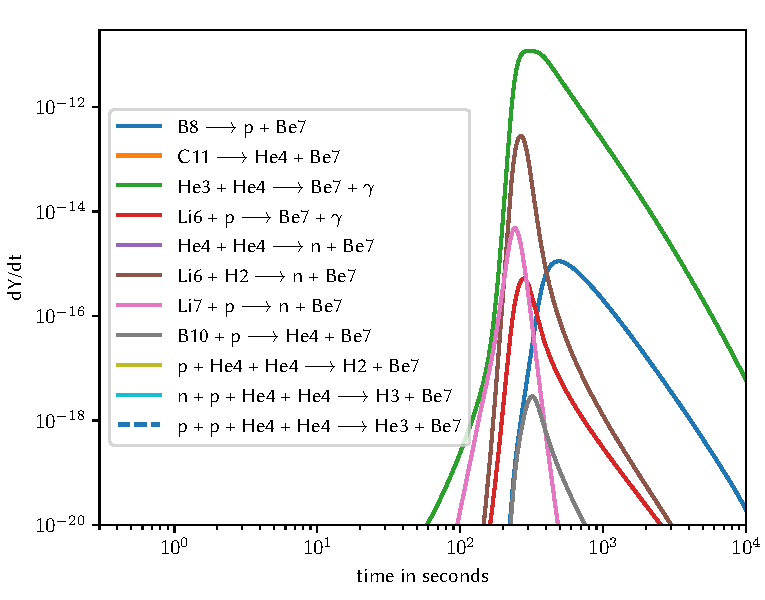
\includegraphics[width=5.1in]{figures/app/Be7create.pdf}
    \caption{Strength of different ${}^7$ Be creation rates}
    \label{fig:Be7create}
\end{figure}

\begin{figure}[ht]
    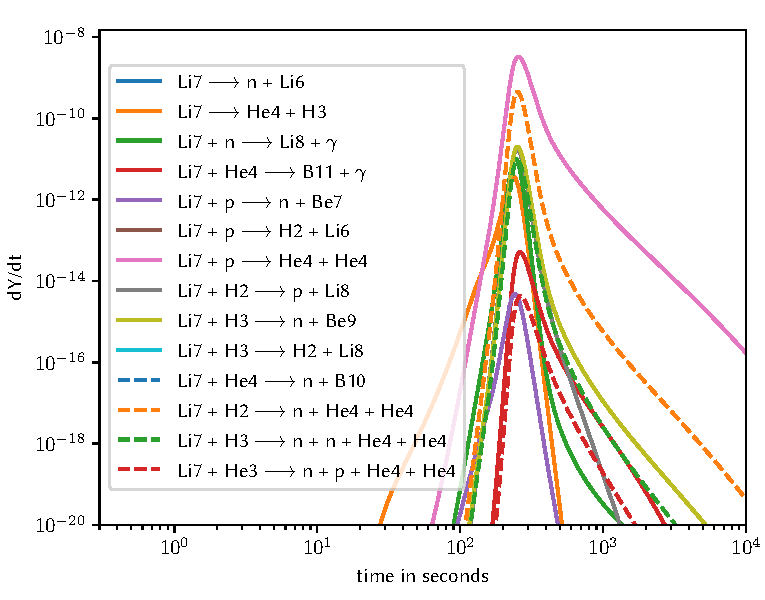
\includegraphics[width=5.1in]{figures/app/Li7destruct.pdf}
    \caption{Strength of different ${}^7$ Li destruction rates}
    \label{fig:Li7destruct}
\end{figure}

\begin{figure}[ht]
    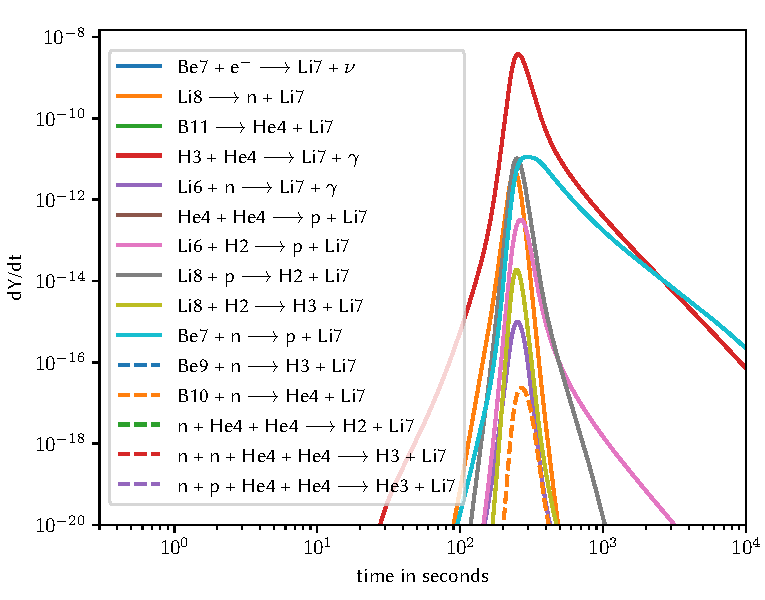
\includegraphics[width=5.1in]{figures/app/Li7create.pdf}
    \caption{Strength of different ${}^7$ Li creation rates}
    \label{fig:Li7create}
\end{figure}

\end{document}